% !TeX root = document.tex
% !TeX encoding = UTF-8 Unicode

\section{Introduction}%
\label{Introduction}
The objective of this report is to show the derivation, analysis, and simulation of a ball on an incline with a magnet in series and the application of PID-based control system with the goal of having the system position the ball within desired position.

\begin{figure}[H]
	\centering
	\captionsetup{justification=centering}
	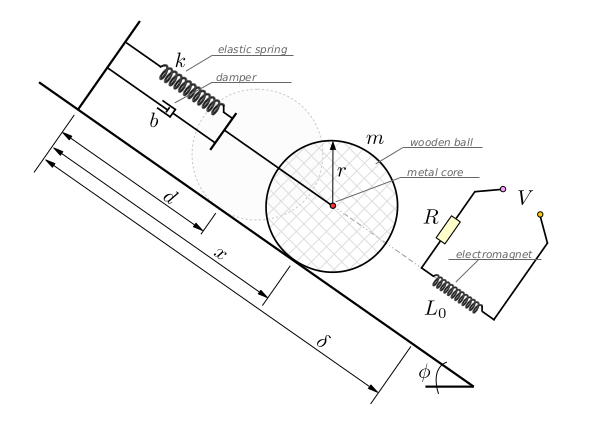
\includegraphics[width=0.8\linewidth]{imgs/problemFigure.png}
	\caption{System of a wooden ball on an inclined plane. Ball attracted downwards by electromagnet, which is controlled by a voltage, V.}%
	\label{fig:14}
\end{figure}


Assignment done in Anaconda, package manager and environment management system. Written in Python language.\\ The libraries imported necessary to complete task: \href{https://anaconda.org/conda-forge/control}{control}, \href{https://anaconda.org/anaconda/sympy}{sympy}, \href{https://anaconda.org/anaconda/numpy}{numpy}, \href{https://anaconda.org/conda-forge/matplotlib}{matplotlib} \\

Completed and functioning code can be found \href{https://github.com/ELE2024-Controls/Coursework}{[here]}. Function and class included within the file, no additional repositories required.